\chapter{Specifikacija programske potpore}
		
	\section{Funkcionalni zahtjevi}
			
			\noindent \textbf{Dionici:}
			
			\begin{packed_enum}
				
				\item Organizator konferencije (naručitelj)
				\item Pokrovitelji konferencije
				\item Autori radova
				\item Glasači
				\item Administrator
				\item Natkorisnik
				\item Razvojni tim
				
			\end{packed_enum}
			
			\noindent \textbf{Aktori i njihovi funkcionalni zahtjevi:}
			
			\begin{packed_enum}
				\item  \underbar{Neregistrirani korisnik (inicijator) može:}
				
				\begin{packed_enum}
					
					\item prijaviti se pomoću generičkog korisničkog računa
					
				\end{packed_enum}
				
				\item  \underbar{Korisnik posjetitelj (inicijator) može:}
				
				\begin{packed_enum}
					
					\item registrirati se, odnosno stvoriti novi korisnički račun
					\item pregledavati postere, pri čemu ne može glasati
					\item vidjeti informacije o vremenu i mjestu održavanja koje uključuju vremenske uvjete, vremensku prognozu i kartu
					
				\end{packed_enum}
			
				\item  \underbar{Registrirani/Prijavljeni korisnik (inicijator) može:}
				
				\begin{packed_enum}
					
					\item pregledati i glasati za postere pri čemu svaki posjetitelj može glasati za najviše jedan poster
					\item pregledavati promotivne materijale pokrovitelja
					\item gledati video-prijenos
					\item pregledati i preuzimati fotografije
					\item pristupiti rezultatima jednom kad postanu dostupni
					\item odjaviti se
				
				\end{packed_enum}
				
				\item  \underbar{Korisnik (inicijator):}
				
				\begin{packed_enum}
					
					\item generalizacija korisnika posjetitelja, registriranog korisnika, administratora i natkorisnika
					\item prijaviti se vlastitim podacima
					
				\end{packed_enum}
				
				\item \underbar{Administrator (inicijator) može:}
				
				\begin{packed_enum}
					
					\item dodati ili ukloniti postere natjecatelja s potrebnim podacima
					\item dodati ili ukloniti fotografije s događaja
					\item dodati ili ukloniti logo pokrovitelja s potrebnim podacima
					\item obrisati određene korisničke račune
					
				\end{packed_enum}
				
				\item \underbar{Natkorisnik (inicijator) može:}
				
				\begin{packed_enum}
					
					\item stvoriti novu konferenciju sa svim podacima potrebnim za njenu funkciju
					\item izbrisati konferenciju

				\end{packed_enum}
				
				\item \underbar{Baza podataka (sudionik):}
				
				\begin{packed_enum}
					
					\item pohranjuje podatke o korisnicima
					\item pohranjuje podatke o digitalnim posterima, broju njihovih glasova, njihovim autorima
					\item pohranjuje fotografije uslikane za vrijeme trajanja konferencije
					\item pohranjuje sve ostale potrebne podatke o konferenciji
					
				\end{packed_enum}
				
				\item \underbar{Poslužitelj strujanja (sudionik):}
				
				\begin{packed_enum}
					
					\item pruža uslugu video prijenosa konferencije
				
				\end{packed_enum}
				
				\item \underbar{Poslužitelj vremenske prognoze (sudionik):}
				
				\begin{packed_enum}
					
					\item poslužuje potrebne podatke vezane za prognozu vremena
					
				\end{packed_enum}
				
				\item \underbar{Poslužitelj karte (sudionik):}
				
				\begin{packed_enum}
					
					\item poslužuje potrebne podatke za prikaz karte
					
				\end{packed_enum}
				
				\item \underbar{Poslužitelj e-pošte (sudionik):}
				
				\begin{packed_enum}
					
					\item omogućuje aplikaciji da šalje e-poruke korisnicima
					
				\end{packed_enum}
				
			\end{packed_enum}
			
			\eject 
			
			
				
			\subsection{Obrasci uporabe}
					
					\newcounter{UseCaseCounter}
					\setcounter{UseCaseCounter}{1}
					
					\noindent \underbar{\textbf{UC\theUseCaseCounter \stepcounter{UseCaseCounter} - Pristup konferenciji}}
					\begin{packed_item}
						
						\item \textbf{Glavni sudionik: } Neregistrirani korisnik
						\item  \textbf{Cilj:} Pristupiti konferenciji kao korisnik posjetitelj
						\item  \textbf{Sudionici:} Baza podataka
						\item  \textbf{Preduvjet:} Nema preduvjeta
						\item  \textbf{Opis osnovnog tijeka:}
						
						\item[] \begin{packed_enum}
							
							\item Korisnik odabire konferenciju kojoj želi pristupiti
							\item Upisuje generičko korisničko ime (predviđenu adresu e-pošte) i lozinku za odabranu konferenciju
							\item Otvara se pregled konferencije s mogućnostima korisnika posjetitelja
						\end{packed_enum}
						
						\item  \textbf{Opis mogućih odstupanja:}
						
						\item[] \begin{packed_item}
							
							\item[2.a] Pogrešno generičko ime ili lozinka
							\item[] \begin{packed_enum}
								
								\item Sustav obavještava korisnika o upisu pogrešne lozinke ili imena
								
							\end{packed_enum}
							
						\end{packed_item}
					\end{packed_item}
					
					\noindent \underbar{\textbf{UC\theUseCaseCounter \stepcounter{UseCaseCounter} - Registracija}}
					\begin{packed_item}
						
						\item \textbf{Glavni sudionik: } Korisnik posjetitelj
						\item  \textbf{Cilj:} Stvoriti vlastiti korisnički račun
						\item  \textbf{Sudionici:} Baza podataka
						\item  \textbf{Preduvjet:} Korisnik je prijavljen s generičkim računom
						\item  \textbf{Opis osnovnog tijeka:}
						
						\item[] \begin{packed_enum}
							
							\item Korisnik odabire opciju za registraciju
							\item Korisnik unosi potrebne korisničke podatke
							\item Korisnik prima obavijest o uspješnoj registraciji
							
						\end{packed_enum}
						
						\item  \textbf{Opis mogućih odstupanja:}
						
						\item[] \begin{packed_item}
							
							\item[2.a] Odabir već zauzete adrese e-pošte, unos korisničkog podatka u nedozvoljenom formatu ili pružanje neispravne adrese e-pošte
							\item[] \begin{packed_enum}
								
								\item Sustav obavještava korisnika o neuspjelom upisu
								\item Korisnik mijenja potrebne podatke te završava unos ili odustaje od registracije
								
							\end{packed_enum}
							
						\end{packed_item}
					\end{packed_item}
					
					\noindent \underbar{\textbf{UC\theUseCaseCounter \stepcounter{UseCaseCounter} - Prijava}}
					\begin{packed_item}
						
						\item \textbf{Glavni sudionik: } Registrirani korisnik
						\item  \textbf{Cilj:} Pristup svim korisničkim funkcionalnostima aplikacije
						\item  \textbf{Sudionici:} Baza podataka
						\item  \textbf{Preduvjet:} Nema preduvjeta
						\item  \textbf{Opis osnovnog tijeka:}
						
						\item[] \begin{packed_enum}
							
							\item Korisnik pritišće gumb za pristup konferenciji ili gumb za prijavu unutar konferencije
							\item Otvara se prozor u koji korisnik upisuje podatke
							\item Provjera postoji li korisnik u bazi podataka kao registrirani korisnik
							\item Ako korisnik postoji, otvara se prozor s podacima o konferenciji, a korisnik je prijavljen
							
						\end{packed_enum}
						
						\item  \textbf{Opis mogućih odstupanja:}
						
						\item[] \begin{packed_item}
							
							\item[1.a] Korisnik pritišće gumb za prijavu natkorisnika
							\item[] \begin{packed_enum}
								
								\item Korisnik unosi natkorisničke podatke
								\item Otvara se natkorisnički prikaz stranice s popisom konferencija
								
							\end{packed_enum}
							
							\item[3.a] Korisnik je Administrator
							\item[] \begin{packed_enum}
								
								\item Korisnik ulazi u aplikaciju s administratorskim ovlastima
								
							\end{packed_enum}
							
							\item[4.a] Korisnik ne postoji u bazi podataka
							\item[] \begin{packed_enum}
								
								\item Sustav obavještava korisnika o upisu pogrešne lozinke ili adrese e-pošte
								
							\end{packed_enum}
							
						\end{packed_item}
					\end{packed_item}
					
					\noindent \underbar{\textbf{UC\theUseCaseCounter \stepcounter{UseCaseCounter} - Odjava}}
					\begin{packed_item}
						
						\item \textbf{Glavni sudionik: } Registrirani korisnik
						\item  \textbf{Cilj:} Odjaviti se iz konferencije
						\item  \textbf{Sudionici:} Baza podataka
						\item  \textbf{Preduvjet:} Korisnik je prijavljen
						\item  \textbf{Opis osnovnog tijeka:}
						
						\item[] \begin{packed_enum}
							
							\item Korisnik odabire opciju za odjavu
							\item Povratak na zaslon za pristup konferenciji
							
						\end{packed_enum}
					\end{packed_item}
					
					\noindent \underbar{\textbf{UC\theUseCaseCounter \stepcounter{UseCaseCounter} - Pregled informacija o konferenciji}}
					\begin{packed_item}
						
						\item \textbf{Glavni sudionik: } Registrirani korisnik
						\item  \textbf{Cilj:} Pregledati informacije o mjestu održavanja konferencije, uključujući kartu i informacije o trenutnim vremenskim uvjetima i vremenskoj prognozi za navedenu lokaciju
						\item  \textbf{Sudionici:} Baza podataka
						\item  \textbf{Preduvjet:} Korisnik je registriran i prijavljen
						\item  \textbf{Opis osnovnog tijeka:}
						
						\item[] \begin{packed_enum}
							
							\item Korisnik se upravo prijavljuje ili pritišće gumb "Konferencija"
							\item Otvara se stranica s podacima o konferenciji
							
						\end{packed_enum}
					\end{packed_item}
					
					\noindent \underbar{\textbf{UC\theUseCaseCounter \stepcounter{UseCaseCounter} - Prikaz video prijenosa}}
					\begin{packed_item}
						
						\item \textbf{Glavni sudionik: } Registrirani korisnik
						\item  \textbf{Cilj:} Gledati video prijenos konferencije
						\item  \textbf{Sudionici:} Poslužitelj strujanja
						\item  \textbf{Preduvjet:} Korisnik je registriran i prijavljen
						\item  \textbf{Opis osnovnog tijeka:}
						
						\item[] \begin{packed_enum}
							
							\item Korisnik otvara prozor s podacima o konferenciji
							\item Pokreće se prijenos videa
							
						\end{packed_enum}
					\end{packed_item}
					
					\noindent \underbar{\textbf{UC\theUseCaseCounter \stepcounter{UseCaseCounter} - Pregled galerije postera}}
					\begin{packed_item}
						
						\item \textbf{Glavni sudionik: } Korisnik
						\item  \textbf{Cilj:} Pregled svih postavljenih postera
						\item  \textbf{Sudionici:} Baza podataka
						\item  \textbf{Preduvjet:} Korisnik je prijavljen
						\item  \textbf{Opis osnovnog tijeka:}
						
						\item[] \begin{packed_enum}
							
							\item Korisnik pritišće gumb "Posteri"
							\item Otvara se prozor s posterima
							
						\end{packed_enum}
						
					\end{packed_item}
					
					\noindent \underbar{\textbf{UC\theUseCaseCounter \stepcounter{UseCaseCounter} - Pregled digitalnog postera/prezentacije}}
					\begin{packed_item}
						
						\item \textbf{Glavni sudionik: } Korisnik
						\item  \textbf{Cilj:} Pregledati poster
						\item  \textbf{Sudionici:} Baza podataka
						\item  \textbf{Preduvjet:} Pregled galerije postera
						\item  \textbf{Opis osnovnog tijeka:}
						
						\item[] \begin{packed_enum}
							
							\item Korisnik odabire digitalni poster
							\item Korisnik pregledava poster/prezentaciju u .pdf formatu
							
						\end{packed_enum}
					\end{packed_item}
					
					\noindent \underbar{\textbf{UC\theUseCaseCounter \stepcounter{UseCaseCounter} - Glasovanje}}
					\begin{packed_item}
						
						\item \textbf{Glavni sudionik: } Registrirani korisnik
						\item  \textbf{Cilj:} Glasovati za rad
						\item  \textbf{Sudionici:} Baza podataka
						\item  \textbf{Preduvjet:} Prijava, Pregled digitalnog postera
						\item  \textbf{Opis osnovnog tijeka:}
						
						\item[] \begin{packed_enum}
							
							\item Korisnik odabire opciju glasovanja
							\item U sustavu se evidentira korisnikovo glasovanje
							
						\end{packed_enum}
						
						\item  \textbf{Opis mogućih odstupanja:}
						
						\item[] \begin{packed_item}
							
							\item[2.a] Korisnik je već glasovao
							\item[] \begin{packed_enum}
								
								\item Korisnik je obaviješten o nemogućnosti daljnjeg glasovanja
								
							\end{packed_enum}
						\end{packed_item}
					\end{packed_item}
					
					\noindent \underbar{\textbf{UC\theUseCaseCounter \stepcounter{UseCaseCounter} - Pregled rezultata glasovanja}}
					\begin{packed_item}
						
						\item \textbf{Glavni sudionik: } Registrirani korisnik
						\item  \textbf{Cilj:} Uvid u rezultate glasovanja
						\item  \textbf{Sudionici:} Baza podataka
						\item  \textbf{Preduvjet:} Prijava, registrirani korisnik
						\item  \textbf{Opis osnovnog tijeka:}
						
						\item[] \begin{packed_enum}
							
							\item Korisnik odabire opciju rezultati glasovanja u izborniku
							\item Otvara se zasebna stranica gdje je rang lista autora/radova
							\item Korisnik pregledava rang listu
						\end{packed_enum}
						
					\end{packed_item}
					
					\noindent \underbar{\textbf{UC\theUseCaseCounter \stepcounter{UseCaseCounter} - Pregled galerije fotografija}}
					\begin{packed_item}
						
						\item \textbf{Glavni sudionik: } Registrirani korisnik
						\item  \textbf{Cilj:} Pregledati galeriju fotografija
						\item  \textbf{Sudionici:} Baza podataka
						\item  \textbf{Preduvjet:} Korisnik je registriran i prijavljen
						\item  \textbf{Opis osnovnog tijeka:}
						
						\item[] \begin{packed_enum}
							
							\item Korisnik pritišće gumb "Fotografije"
							\item Otvara se galerija fotografija
							
						\end{packed_enum}
					\end{packed_item}
					
					\noindent \underbar{\textbf{UC\theUseCaseCounter \stepcounter{UseCaseCounter} - Pregled fotografije}}
					\begin{packed_item}
						
						\item \textbf{Glavni sudionik: } Registrirani korisnik
						\item  \textbf{Cilj:} Pregledati izabranu fotografiju iz galerije fotografija
						\item  \textbf{Sudionici:} Baza podataka
						\item  \textbf{Preduvjet:} Posjetitelj je prijavljen te je otvorena galerija fotografija
						\item  \textbf{Opis osnovnog tijeka:}
						
						\item[] \begin{packed_enum}
							
							\item Korisnik odabire fotografiju iz galerije
							\item Odabrana fotografije prikaže se uvećana
							
						\end{packed_enum}
					\end{packed_item}
					
					\noindent \underbar{\textbf{UC\theUseCaseCounter \stepcounter{UseCaseCounter} - Preuzimanje fotografije}}
					\begin{packed_item}
						
						\item \textbf{Glavni sudionik: } Registrirani korisnik
						\item  \textbf{Cilj:} Preuzeti izabranu fotografiju iz galerije
						\item  \textbf{Sudionici:} Baza podataka
						\item  \textbf{Preduvjet:} Posjetitelj je prijavljen, otvorena je galerija fotografija, galerija nije prazna
						\item  \textbf{Opis osnovnog tijeka:}
						
						\item[] \begin{packed_enum}
							
							\item Korisnik odabire opciju za preuzimanje fotografije
							\item Odabrana fotografija se preuzima na uređaj
							
						\end{packed_enum}
						
					\end{packed_item}
					
					\noindent \underbar{\textbf{UC\theUseCaseCounter \stepcounter{UseCaseCounter} - Pregled promotivnih materijala}}
					\begin{packed_item}

						\item \textbf{Glavni sudionik: } Registrirani korisnik
						\item  \textbf{Cilj:} Pregledati promotivne materijale pokrovitelja konferencije
						\item  \textbf{Sudionici:} Baza podataka
						\item  \textbf{Preduvjet:} Korisnik je registriran i prijavljen
						\item  \textbf{Opis osnovnog tijeka:}
						
						\item[] \begin{packed_enum}
							
							\item Korisnik pritišće gumb "Pokrovitelji"
							\item Otvara se stranica s promotivnim materijalima

						\end{packed_enum}

					\end{packed_item}
					
					\noindent \underbar{\textbf{UC\theUseCaseCounter \stepcounter{UseCaseCounter} - Brisanje korisničkog računa}}
					\begin{packed_item}
						
						\item \textbf{Glavni sudionik: }Administrator
						\item  \textbf{Cilj:} Izbrisati korisnički račun
						\item  \textbf{Sudionici:} Baza podataka
						\item  \textbf{Preduvjet:} Administrator je prijavljen
						\item  \textbf{Opis osnovnog tijeka:}
						
						\item[] \begin{packed_enum}
							
							\item Administrator otvori popis registriranih korisnika
							\item Administrator pritišće gumb "Ukloni"
							\item Podaci o odabranom korisniku se brišu iz baze podataka
							
						\end{packed_enum}
					\end{packed_item}
					
					\noindent \underbar{\textbf{UC\theUseCaseCounter \stepcounter{UseCaseCounter} - Dodavanje digitalnog postera}}
					\begin{packed_item}
						
						\item \textbf{Glavni sudionik: } Administrator
						\item  \textbf{Cilj:} Dodavanje novog postera
						\item  \textbf{Sudionici:} Baza Podataka
						\item  \textbf{Preduvjet:} Administrator je prijavljen, otvoren je administratorov prikaz galerije postera
						\item  \textbf{Opis osnovnog tijeka:}
						
						\item[] \begin{packed_enum}
							
							\item Administrator pritišće gumb za dodavanje novog postera
							\item Otvara se prozor s mogućnošću odabira lokalne datoteke i unosa podataka o posteru
							\item Administrator odabire željenu datoteku za prijenos u bazu podataka aplikacije
							\item Administrator potvrđuje dodavanje novog postera
							\item Podaci o novom posteru se spremaju u bazu podataka
							
						\end{packed_enum}
						
						\item  \textbf{Opis mogućih odstupanja:}
						
						\item[] \begin{packed_item}
							
							\item[3.a] Odabrana datoteka nije u .pdf formatu
							\item[] \begin{packed_enum}
								
								\item Sustav obavještava administratora o odabiru datoteke nepodržanog tipa
								\item Odbacivanje promjena
								
							\end{packed_enum}			
						\end{packed_item}
					\end{packed_item}
					
					\noindent \underbar{\textbf{UC\theUseCaseCounter \stepcounter{UseCaseCounter} - Brisanje digitalnog postera}}
					\begin{packed_item}
						
						\item \textbf{Glavni sudionik: } Administrator
						\item  \textbf{Cilj:} Brisanje odabranog digitalnog postera
						\item  \textbf{Sudionici:} Baza podataka
						\item  \textbf{Preduvjet:} Administrator je prijavljen, otvoren je administratorov prikaz galerije postera
						\item  \textbf{Opis osnovnog tijeka:}
						
						\item[] \begin{packed_enum}
							
							\item Administrator pritišće gumb "Obriši" ispod odabranog postera
							\item Podaci o odabranom posteru se brišu iz baze podataka, a on se više ne vidi u galeriji
							
						\end{packed_enum}
					\end{packed_item}
					
					\noindent \underbar{\textbf{UC\theUseCaseCounter \stepcounter{UseCaseCounter} - Dodavanje fotografije}}
					\begin{packed_item}
						
						\item \textbf{Glavni sudionik: }Administrator
						\item  \textbf{Cilj:} Dodavanje nove fotografije u galeriju fotografija
						\item  \textbf{Sudionici:} Baza podataka
						\item  \textbf{Preduvjet:} Prijavljen je administrator, otvoren je administratorov prikaz galerije fotografija
						\item  \textbf{Opis osnovnog tijeka:}
						
						\item[] \begin{packed_enum}
							
							\item Administrator pritišće gumb za dodavanje nove fotografije
							\item Otvara se prozor s poljem za unos lokalne datoteke
							\item Administrator odabire sliku s vlastitog računala
							\item Administrator potvrđuje postavljanje nove fotografije
							\item Podaci o novoj fotografiji se spremaju u bazu podataka

						\end{packed_enum}
						
						\item  \textbf{Opis mogućih odstupanja:}
						
						\item[] \begin{packed_item}
							
							\item[3.a] Odabrana datoteka nije podržanog tipa
							\item[] \begin{packed_enum}
								
								\item Sustav obavještava administratora o odabiru datoteke nepodržanog tipa
								\item Odbacivanje promjena
								
							\end{packed_enum}
						\end{packed_item}
					\end{packed_item}
					
					\noindent \underbar{\textbf{UC\theUseCaseCounter \stepcounter{UseCaseCounter} - Brisanje fotografije}}
					\begin{packed_item}
						
						\item \textbf{Glavni sudionik: }Administrator
						\item  \textbf{Cilj:} Brisanje odabrane fotografije
						\item  \textbf{Sudionici:} Baza podataka
						\item  \textbf{Preduvjet:} Prijavljen je administrator, otvoren je administratorov prikaz galerije fotografija
						\item  \textbf{Opis osnovnog tijeka:}
						
						\item[] \begin{packed_enum}
							
							\item Administrator odabire fotografiju
							\item Otvara se uvećani prikaz fotografije
							\item Administrator odabire gumb za brisanje fotografije
							\item Podaci o fotografiji se miču iz baze podataka i fotografija se miče iz galerije
							
						\end{packed_enum}
					\end{packed_item}
					
					\noindent \underbar{\textbf{UC\theUseCaseCounter \stepcounter{UseCaseCounter} - Dodavanje promotivnog materijala}}
					\begin{packed_item}
						
						\item \textbf{Glavni sudionik: }Administrator
						\item  \textbf{Cilj:} Dodati novi promotivni materijal
						\item  \textbf{Sudionici:} Baza podataka
						\item  \textbf{Preduvjet:} Prijavljen je administrator, otvoren je administratorov prikaz promotivnih materijala
						\item  \textbf{Opis osnovnog tijeka:}
						
						\item[] \begin{packed_enum}
							
							\item Administrator pritišće gumb za dodavanje novog promotivnog materijala
							\item Administrator unosi potrebne podatke i lokalnu datoteku sa znakom pokrovitelja
							\item Administrator potvrđuje promjene
							\item Podaci o pokrovitelju se unose u bazu podataka
							
						\end{packed_enum}
						
						\item  \textbf{Opis mogućih odstupanja:}
						
						\item[] \begin{packed_item}
							
							\item[2.a] Odabrana datoteka nije podržanog tipa
							\item[] \begin{packed_enum}
								
								\item Sustav obavještava administratora o odabiru datoteke nepodržanog tipa
								\item Odbacivanje promjena
								
							\end{packed_enum}
							
						\end{packed_item}
					\end{packed_item}
					
					\noindent \underbar{\textbf{UC\theUseCaseCounter \stepcounter{UseCaseCounter} - Brisanje promotivnog materijala}}
					\begin{packed_item}
						
						\item \textbf{Glavni sudionik: }Administrator
						\item  \textbf{Cilj:} Brisanje odabranog promotivnog materijala
						\item  \textbf{Sudionici:} Baza podataka
						\item  \textbf{Preduvjet:} Prijavljen je administrator, otvoren je administratorov prikaz promotivnih materijala
						\item  \textbf{Opis osnovnog tijeka:}
						
						\item[] \begin{packed_enum}
							
							\item Administrator pritišće gumb "Obriši" ispod odabranog logotipa pokrovitelja
							\item Podaci o odabranom pokrovitelju se brišu iz baze podataka i logotip se više ne vidi na stranici
							
						\end{packed_enum}
						
						\item  \textbf{Opis mogućih odstupanja:}
						
						\item[] \begin{packed_item}
							
							\item[2.a] Administrator odustaje od brisanja materijala
							\item[] \begin{packed_enum}
								
								\item Povratak na sučelje za upravljanje promotivnim materijalima
								
							\end{packed_enum}
							
						\end{packed_item}
					\end{packed_item}
					
					\noindent \underbar{\textbf{UC\theUseCaseCounter \stepcounter{UseCaseCounter} - Dohvat vremenske prognoze}}
					\begin{packed_item}
						
						\item \textbf{Glavni sudionik: } Poslužitelj vremenske prognoze
						\item  \textbf{Cilj:} Dohvatiti podatke o vremenskoj prognozi
						\item  \textbf{Sudionici:} -
						\item  \textbf{Preduvjet:} Prijavljen je registrirani korisnik, aplikacija je pokrenuta
						\item  \textbf{Opis osnovnog tijeka:}
						
						\item[] \begin{packed_enum}
							
							\item Nakon prijave registriranog korisnika aplikacija šalje zahtjev za podacima poslužitelju vremenske prognoze
							
						\end{packed_enum}
					\end{packed_item}	
					
						\noindent \underbar{\textbf{UC\theUseCaseCounter \stepcounter{UseCaseCounter} - Dohvat karte}}
					\begin{packed_item}
						
						\item \textbf{Glavni sudionik: } Poslužitelj karte
						\item  \textbf{Cilj:} Dohvatiti kartu
						\item  \textbf{Sudionici:} -
						\item  \textbf{Preduvjet:} Prijavljen je registrirani korisnik, aplikacija je pokrenuta
						\item  \textbf{Opis osnovnog tijeka:}
						
						\item[] \begin{packed_enum}
							
							\item Nakon prijave registriranog korisnika aplikacija šalje zahtjev za podacima poslužitelju karte
							
						\end{packed_enum}
					\end{packed_item}	
					
					\noindent \underbar{\textbf{UC\theUseCaseCounter \stepcounter{UseCaseCounter} - Slanje poruke e-pošte}}
					\begin{packed_item}
						
						\item \textbf{Glavni sudionik: } Poslužitelj e-pošte
						\item  \textbf{Cilj:} Poslati poruku e-pošte
						\item  \textbf{Sudionici:} Baza podataka
						\item  \textbf{Preduvjet:} Završen postupak glasovanja
						\item  \textbf{Opis osnovnog tijeka:}
						
						\item[] \begin{packed_enum}
							
							\item Traženje i dohvat adresa e-pošte autora prvih triju radova po broju glasova iz baze podataka
							\item Slanje poziva na dodjelu nagrade autorima nagrađenih radova e-porukom i notifikacijom na aplikaciji
							\item Slanje obavijesti o mjestu i vremenu dodjele nagrade svim registriranim korisnicima e-porukom i notifikacijom na aplikaciji
							\item Dohvaćanje adresa e-pošte svih autora natjecateljskih radova
							\item Slanje obavijesti o rangu svim sudionicima natjecanja e-porukom i notifikacijom na aplikaciji
						\end{packed_enum}
						
					\end{packed_item}
					
					\noindent \underbar{\textbf{UC\theUseCaseCounter \stepcounter{UseCaseCounter} - Dodavanje konferencije}}
					\begin{packed_item}
						
						\item \textbf{Glavni sudionik: } Natkorisnik
						\item  \textbf{Cilj:} Stvoriti novu konferenciju
						\item  \textbf{Sudionici:} Baza podataka
						\item  \textbf{Preduvjet:} Prijavljen je natkorisnik, otvoren je natkorisnički prikaz popisa konferencija
						\item  \textbf{Opis osnovnog tijeka:}
						
						\item[] \begin{packed_enum}
							
							\item Natkorisnik odabire opciju za stvaranje nove konferencije
							\item Otvara se obrazac za unos podataka o potrebnih za stvaranje konferencije
							\item Natkorisnik unosi potrebne podatke
							\item Natkorisnik potvrđuje unos podataka
							\item Podaci o novostvorenoj konferenciji se spremaju u bazu podataka
							
						\end{packed_enum}
						
						\item  \textbf{Opis mogućih odstupanja:}
						
						\item[] \begin{packed_item}
							
							\item[4.a] Natkorisnik odustaje od brisanja konferencije
							\item[] \begin{packed_enum}
								
								\item Povratak na popis konferencija
								
							\end{packed_enum}
						\end{packed_item}
					\end{packed_item}
					
					\noindent \underbar{\textbf{UC\theUseCaseCounter \stepcounter{UseCaseCounter} - Brisanje konferencije}}
					\begin{packed_item}
						
						\item \textbf{Glavni sudionik: } Natkorisnik
						\item  \textbf{Cilj:} Izbrisati konferenciju
						\item  \textbf{Sudionici:} Baza podataka
						\item  \textbf{Preduvjet:} Prijavljen je natkorisnik, otvoren je natkorisnički prikaz popisa konferencija
						\item  \textbf{Opis osnovnog tijeka:}
						
						\item[] \begin{packed_enum}
							
							\item Korisnik pritišće gumb "Obriši" pored naziva konferencije koju želi obrisati
							\item Podaci o odabranoj konferenciji se brišu iz baze podataka i njezino ime više nije na popisu konferencija
							
						\end{packed_enum}
					\end{packed_item}
				
				\clearpage
				\subsubsection{Dijagrami obrazaca uporabe}
					
					\begin{figure} [hbt!]
						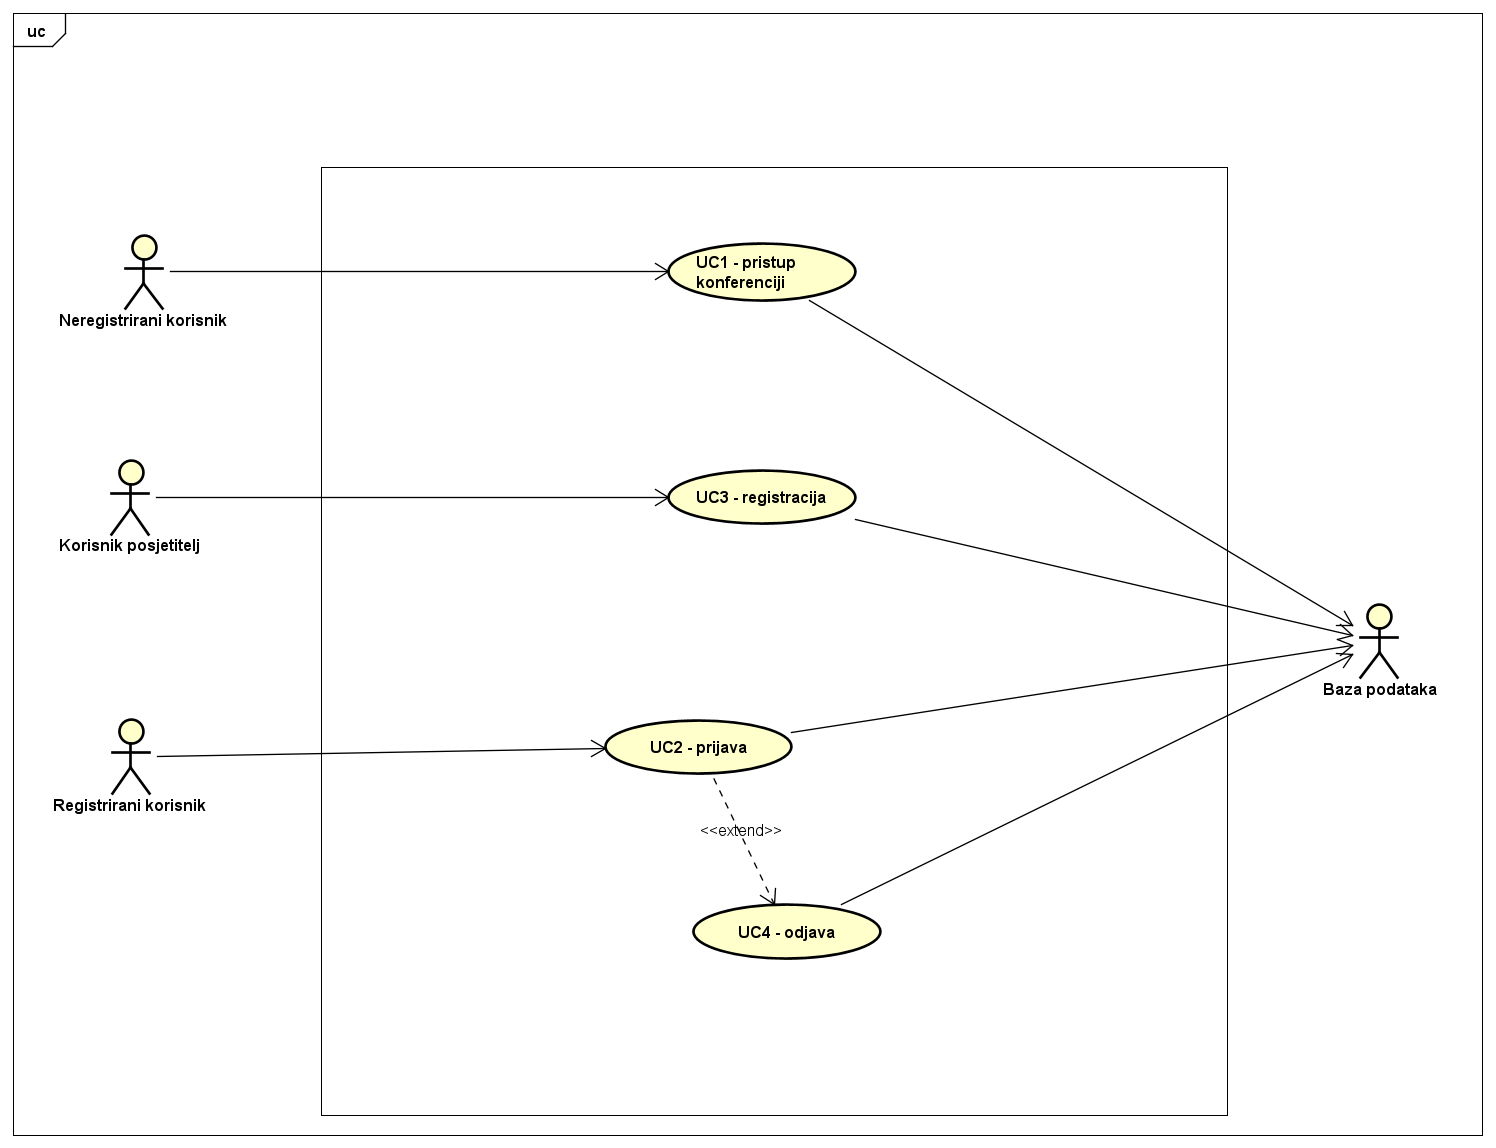
\includegraphics[width=\linewidth]{Slike/UCDiagramUserProfiles.png}
						\caption{UC dijagram za opis korisničkih računa}
					\end{figure}
					
					\begin{figure}
						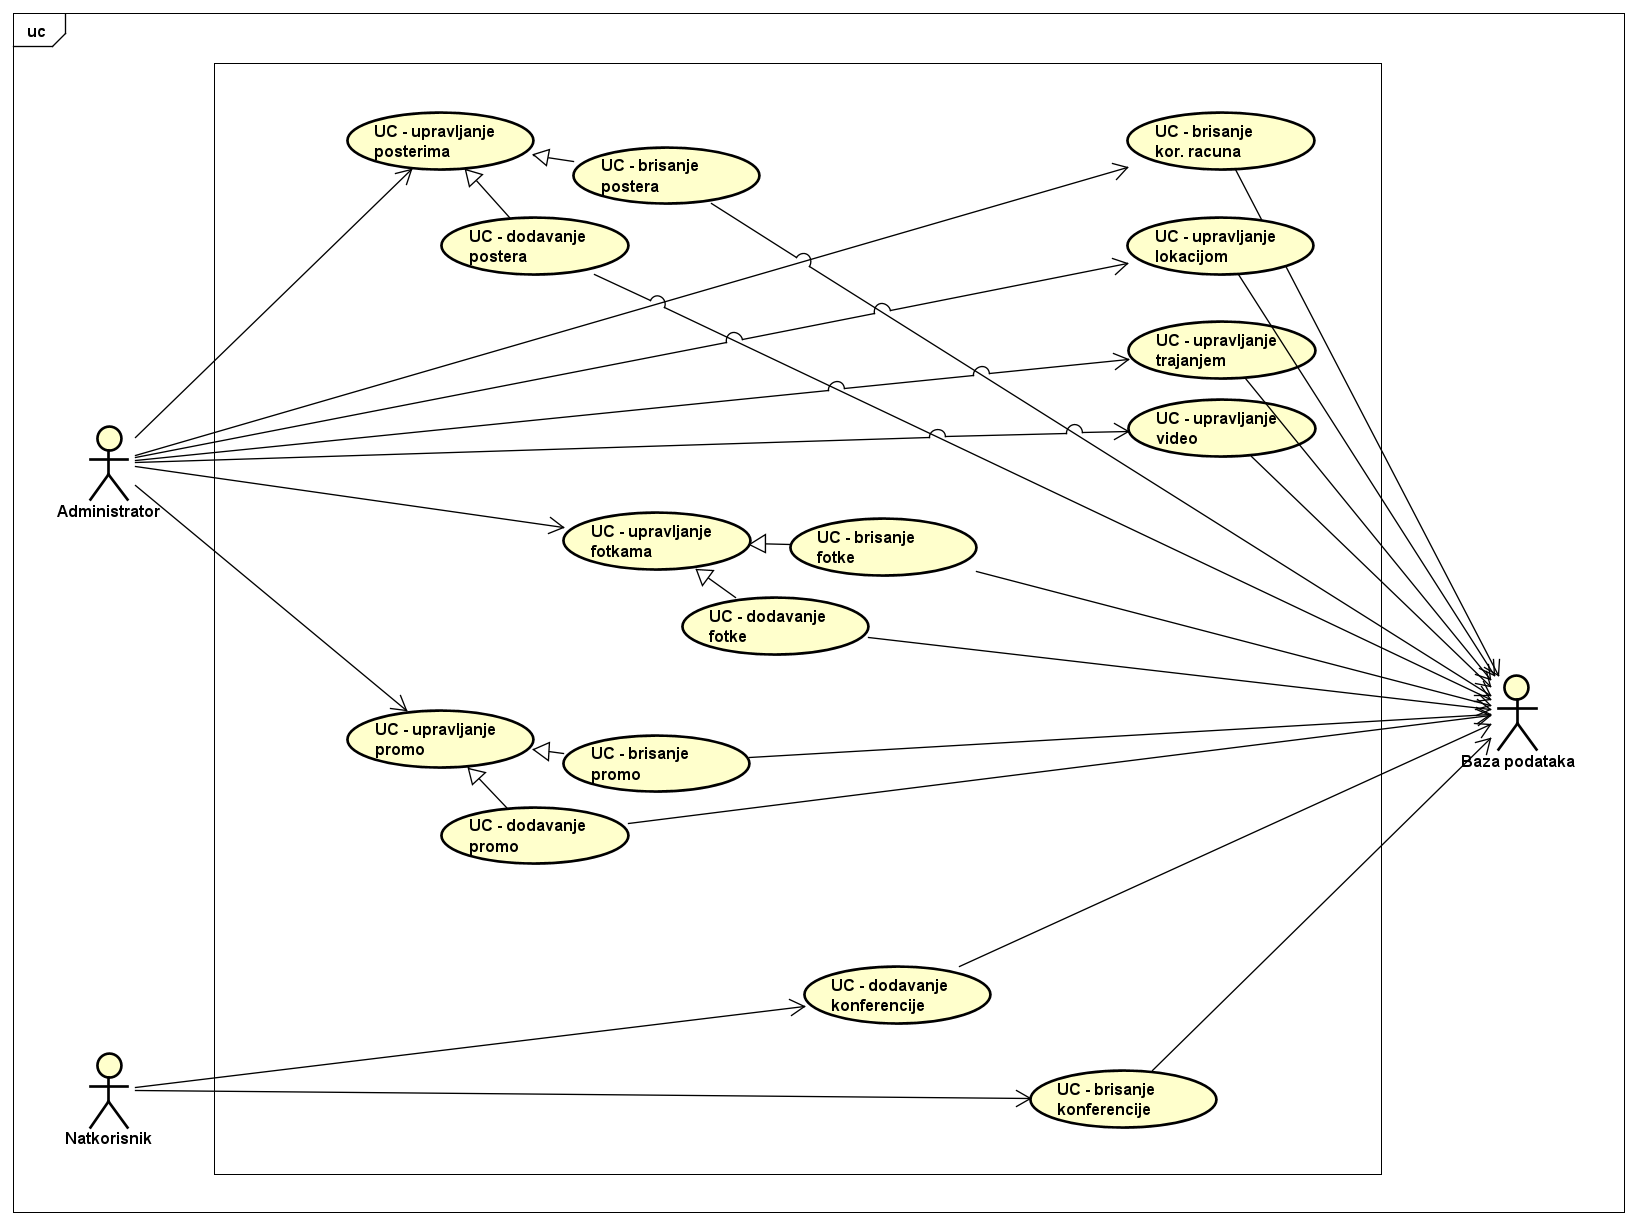
\includegraphics[width=\linewidth]{Slike/UCDiagramAdmin.png}
						\caption{UC dijagram za opis administrativnih mogućnosti}
					\end{figure}
				
					\begin{figure}
						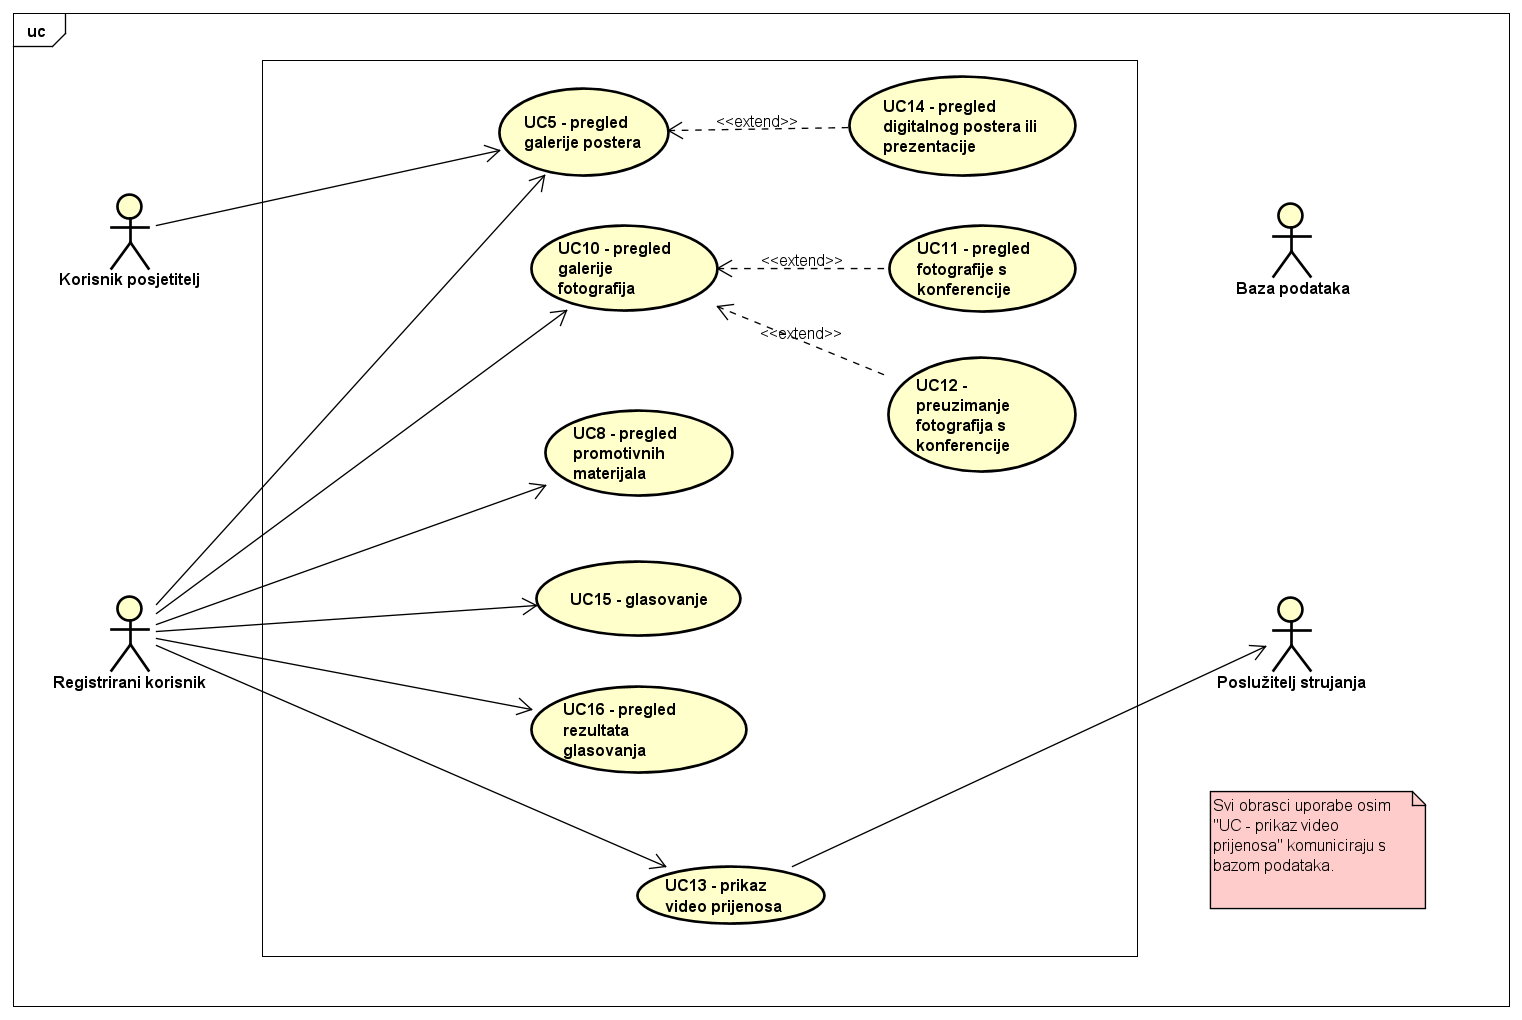
\includegraphics[width=\linewidth]{Slike/UCDiagramAppFunctionalities.png}
						\caption{UC dijagram za opis funkcionalnosti aplikacije}
					\end{figure}
				
				\eject		
			
			\clearpage
			\subsection{Sekvencijski dijagrami}
				
				\subsubsection{Obrazac uporabe UC15 - Glasovanje}
				Registrirani korisnik odabire opciju za pregled svih postera. U galeriji postera odabire jedan poster. Pojavljuje se opcija za glasovanje za odabrani poster. Klikom na tu opciju aplikacija šalje zahtjev bazi podataka kojim provjerava je li prijavljeni korisnik već glasao, te ako jest zabranjuje mu daljnje glasanje. Ukoliko korisnik nije glasao, baza podataka sprema glas. Aplikacija obavještava korisnika o uspješnom glasanju.
				
				\begin{figure}[hp!]
				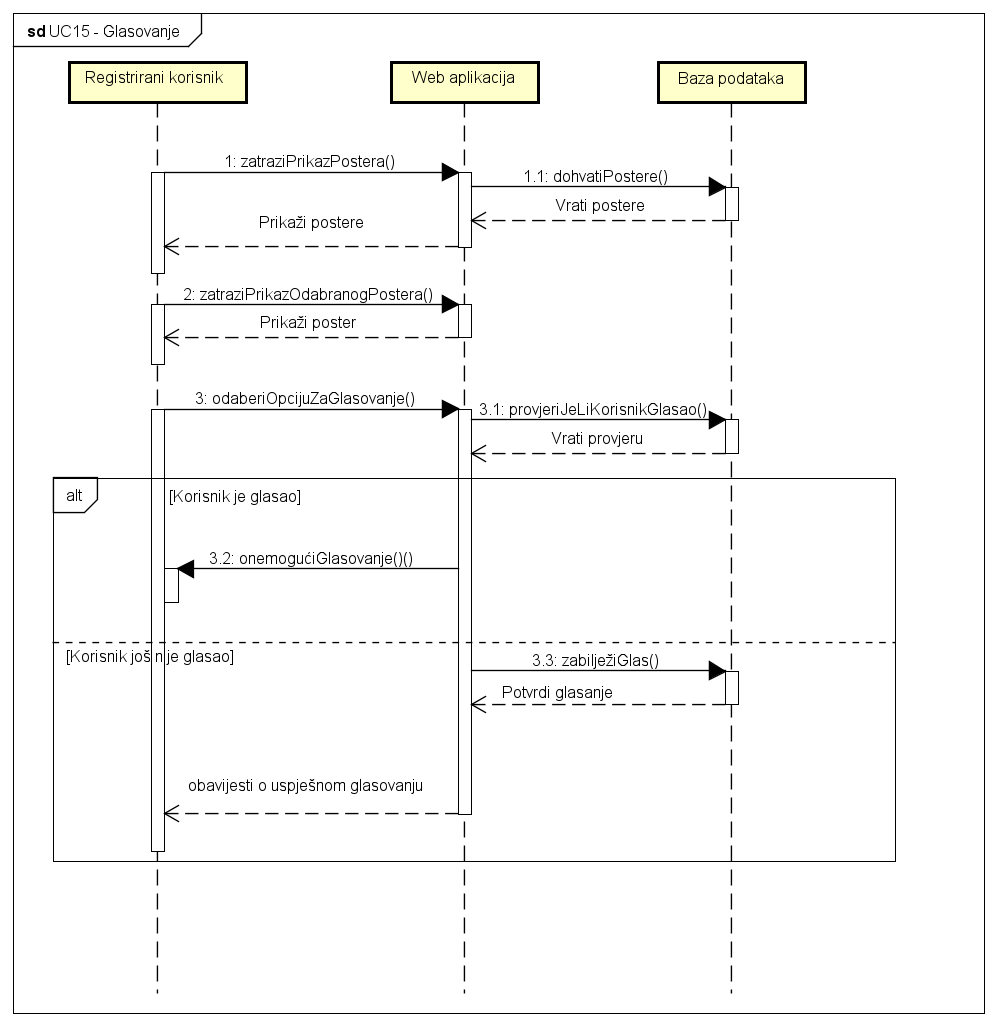
\includegraphics[width=\linewidth]{Slike/SD_Glasanje.png}
				\caption{Sekvencijski dijagram za UC15 - Glasovanje}
				\end{figure}
				
				\newpage
				
				\subsubsection{Obrazac uporabe UC18 - Upravljanje digitalnim posterima}
				Administrator odabire opciju "Galerija postera". Poslužitelj dohvaća popis postera iz baze podataka te ih prikazuje administratoru, kome se uz njih prikazuje i gumb predviđen za upravljanje digitalnim posterima. Pritiskom na njega otvara se posebno sučelje za upravljanje digitalnim posterima koje omogućava dodavanje i brisanje digitalnih postera.
				
				\subsubsection{Obrazac uporabe UC19 - Dodavanje digitalnog postera}
				Administrator pritišće gumb za dodavanje novog postera. Poslužitelj zatraži unos osnovnih podataka o posteru i  prijenos lokalne datoteke postera - administratoru se upit prikazuje kao novo otvoreni prozor. Administrator unosi podatke. Poslužitelj traži potvrdu promjena i čeka odgovor. Nakon potvrde promjena poslužitelj sprema podatke vezane uz poster u bazu podataka, a ona vraća potvrdu izmjene.
				
				\subsubsection{Obrazac uporabe UC20 - Brisanje digitalnog postera}
				Administrator odabire digitalni poster koji želi obrisati. Poslužitelj dohvaća podatke o posteru iz baze podataka. Administrator odabire opciju brisanja digitalnog postera. Poslužitelj šalje upit za potvrdu brisanja. Nakon što administrator potvrdi brisanje postera, poslužitelj ga briše iz baze podataka koja vraća potvrdu izmjene.
				
				\newpage
				
				\begin{figure}[hp!]
					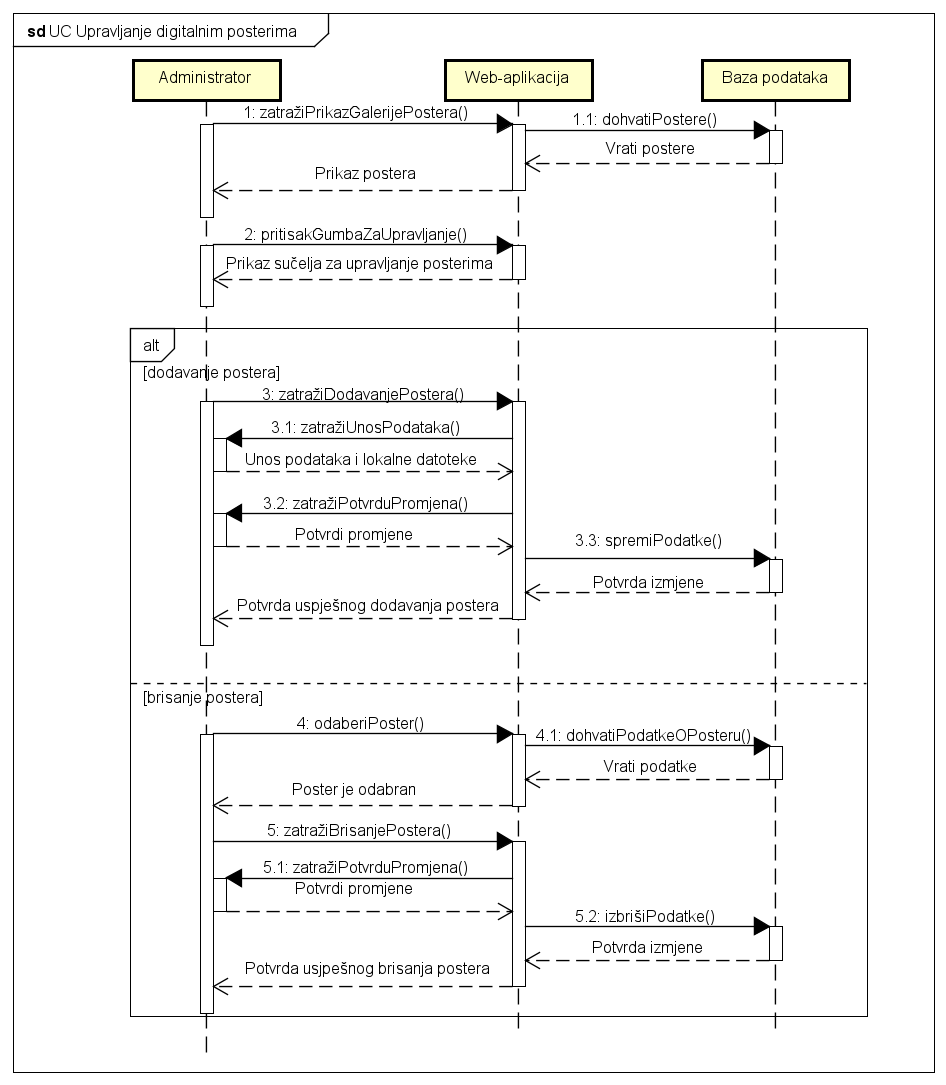
\includegraphics[width=\linewidth]{Slike/SD_UpravljanjePosterima.png}
					\caption{Sekvencijski dijagram za UC18 - Upravljanje posterima}
				\end{figure}
				
				\newpage
				
				\subsubsection{Obrazac uporabe UC31 - Slanje poruke e-pošte}
				Nakon što je glasovanje završeno šalju se tri vrste automatiziranih poruka e-pošte. Prvim trima autorima po broju glasova šalje se poziv na dodjelu nagrade. Svim autorima, bez obzira na njihov rang šalje se poruka o njihovom rangu. Svim registriranim korisnicima šalje se obavijest o mjestu i vremenu dodjele nagrade. Iste poruke se pojavljuju kao obavijesti u aplikaciji.
				
				\begin{figure}[hp!]
					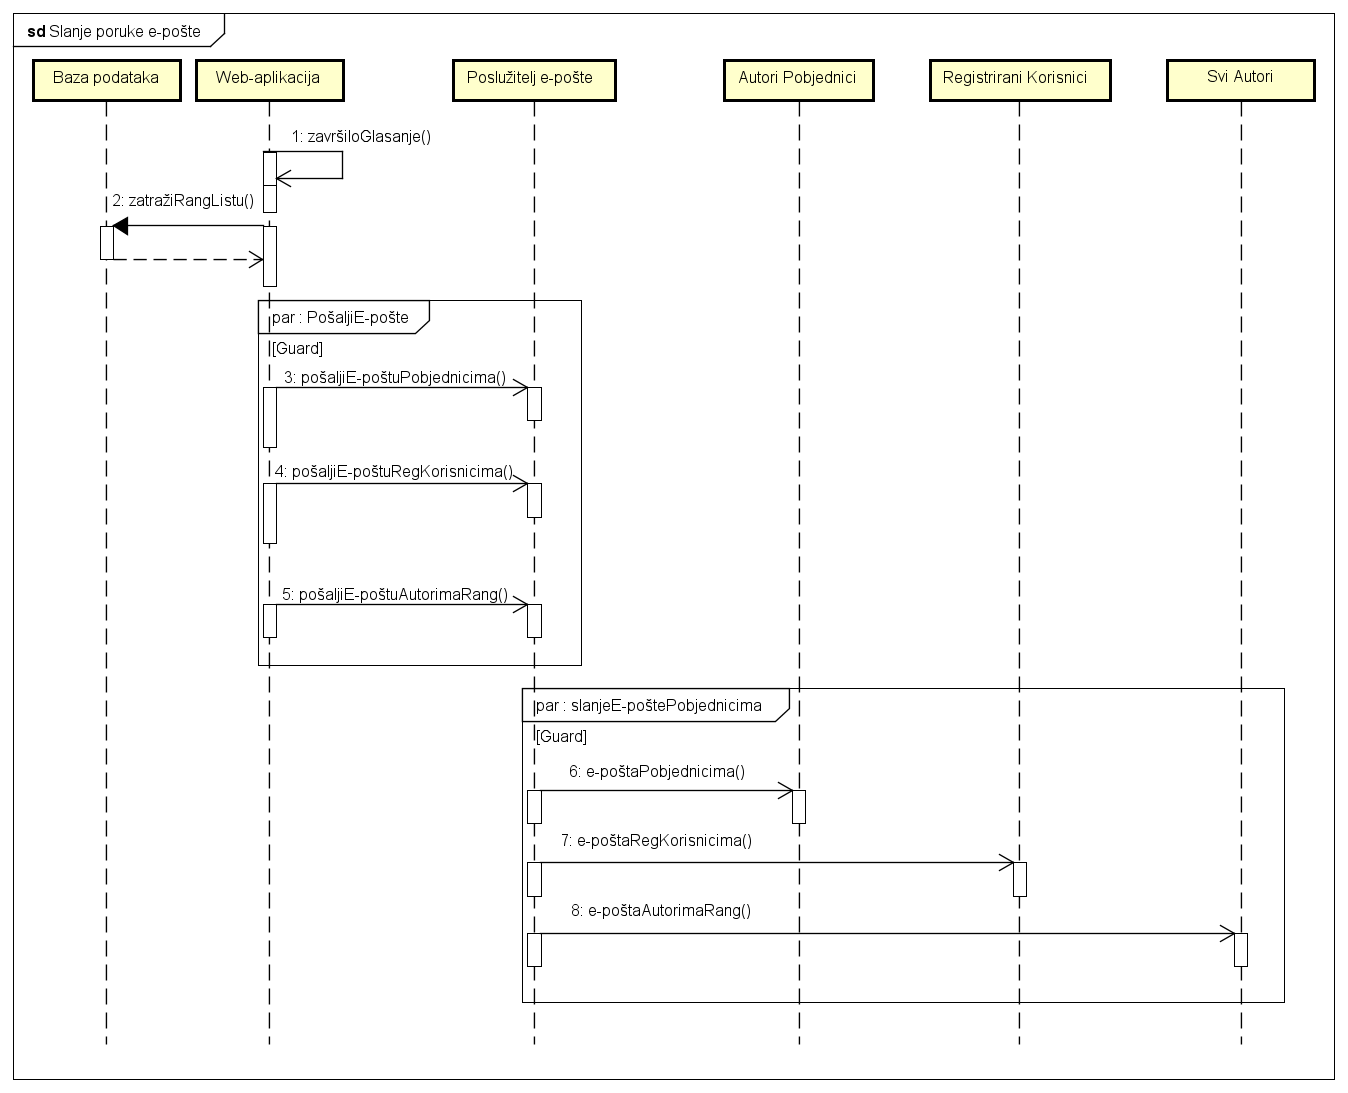
\includegraphics[width=\linewidth]{Slike/SD_SlanjeEPoste.png}
					\caption{Sekvencijski dijagram za UC31 - Slanje e-pošte}
				\end{figure}
				
				\newpage
				
				\eject
			
		\section{Ostali zahtjevi}
		
			 \begin{itemize}
			 	\item Maksimalni broj glasovanja po osobi je 1
			 	\item Glasovanje je moguće samo tijekom određenog vremenskog razdoblja koje je određeno trajanjem konferencije
			 	\item Sustav treba podržavati rad više korisnika u stvarnom vremenu.
			 	\item Korisničko sučelje i sustav moraju podržavati hrvatsku abecedu (dijakritičke
			 	znakove) pri unosu i prikazu tekstualnog sadržaja
			 	\item Izvršavanje dijela programa u kojem se pristupa bazi podataka ne smije trajati dulje od nekoliko sekundi
			 	\item Sustav treba biti implementiran kao web aplikacija koristeći objektno-orijentirane
			 	jezike
			 	\item Neispravno korištenje korisničkog sučelja ne smije narušiti funkcionalnost i rad sustava
			 	\item Sustav treba biti jednostavan za korištenje, korisnici se moraju znati koristiti sučeljem bez opširnih uputa
			 	\item Nadogradnja sustava ne smije narušavati postojeće funkcionalnosti sustava
			 	\item Veza s bazom podataka mora biti kvalitetno zaštićena, brza i otporna na vanjske greške
			 	\item Pristup sustavu mora biti omogućen iz javne mreže protokolom HTTPS
			 \end{itemize}
			 
			 
			 
	